\documentclass[11pt,letterpaper]{article}
% isms-27000-style.tex
% Suite preamble for the ISO/IEC 27000/27001/27002 ISMS engineering suite.
%
% RECONSTRUCTION PROVENANCE: the ten uploaded suite documents load a shared
% preamble with `\input{style.tex}`, but no `style.tex` was present in the
% upload batches or anywhere in this repository's history. This file is a
% documented, suite-specific reconstruction inferred from the macros, colors
% and environments the documents actually use (colors navy/teal/graytext/pale;
% tag commands \SourceTag, \EngineeringTag, \SourceNote{..}; breakable
% tcolorbox callouts; color-striped longtables; TikZ flow diagrams). It is
% NOT the recovered original style; the original visual design is unknown.
%
% pdfLaTeX only.
\usepackage[T1]{fontenc}
\usepackage[utf8]{inputenc}
\usepackage{lmodern}
\usepackage{microtype}
\usepackage[letterpaper,margin=0.9in,headheight=15pt]{geometry}
\usepackage[table]{xcolor}
\definecolor{navy}{HTML}{14355A}
\definecolor{teal}{HTML}{0A7580}
\definecolor{graytext}{HTML}{55616E}
\definecolor{pale}{HTML}{EFF5F7}
\usepackage{amsmath,amssymb}
\usepackage{array,booktabs,longtable,tabularx,multirow}
\usepackage{enumitem}
\usepackage[most]{tcolorbox}
\usepackage{tikz}
\usetikzlibrary{arrows.meta,positioning,shapes.geometric,fit,calc}
\usepackage{needspace}
\usepackage{titlesec}
\usepackage{fancyhdr}
\usepackage{lastpage}
\usepackage{hyperref}
\hypersetup{colorlinks=true,linkcolor=navy,urlcolor=teal,citecolor=navy,pdfauthor={ISMS Engineering Documentation Suite},pdfsubject={Original supporting guidance for ISO/IEC 27000, 27001 and 27002}}
\setlength{\parindent}{0pt}
\setlength{\parskip}{5pt plus 1pt}
\setlength{\emergencystretch}{2em}
\renewcommand{\arraystretch}{1.18}
\setlist[itemize]{itemsep=2pt,topsep=3pt,leftmargin=1.5em}
\setlist[enumerate]{itemsep=2pt,topsep=3pt,leftmargin=1.7em}
\titleformat{\section}{\Large\bfseries\color{navy}}{\thesection}{0.7em}{}[\vspace{-3pt}\color{teal}\titlerule]
\titleformat{\subsection}{\large\bfseries\color{navy}}{\thesubsection}{0.6em}{}
\titleformat{\subsubsection}{\normalsize\bfseries\color{teal}}{\thesubsubsection}{0.55em}{}
\pagestyle{fancy}
\fancyhf{}
\fancyhead[L]{\sffamily\footnotesize ISO/IEC 27000 series | ISMS Engineering}
\fancyhead[R]{\sffamily\footnotesize\color{graytext} Independent companion}
\fancyfoot[L]{\sffamily\scriptsize Original explanatory material; consult the licensed standards}
\fancyfoot[R]{\sffamily\scriptsize\thepage\ / \pageref{LastPage}}
\renewcommand{\headrulewidth}{0.3pt}
% Inline provenance tags used throughout the suite: \SourceTag marks
% statements grounded in the standards; \EngineeringTag marks original
% engineering interpretation. Both are zero-argument label commands.
\newcommand{\SourceTag}{\textsf{\footnotesize\bfseries\color{navy}[Standard]}~}
\newcommand{\EngineeringTag}{\textsf{\footnotesize\bfseries\color{teal}[Engineering]}~}
\newcommand{\SourceNote}[1]{\par\smallskip{\footnotesize\color{graytext}\textit{Trace: #1.}}\par}

\begin{document}
\pagenumbering{roman}
\begin{titlepage}
\vspace*{1.2in}
{\color{teal}\rule{\textwidth}{4pt}}\par\vspace{20pt}
{\Huge\bfseries\color{navy} ISMS Assessment, Audit and Evidence}\par\vspace{18pt}
{\Large\color{graytext} ISO 27001 clause traceability, audit workpapers, assurance and nonconformities}\par\vspace{1.3in}
{\large ISO/IEC 27000:2018 $\vert$ ISO/IEC 27001:2022 $\vert$ ISO/IEC 27002:2022}\par
\vfill
\textbf{Independent educational and engineering implementation reference}\par
Version 1.0 $\cdot$ October 2026\par
{\small Original explanatory material. Source standards are copyrighted; consult licensed originals for authoritative requirements.}\par
\end{titlepage}
\tableofcontents\clearpage\pagenumbering{arabic}
\section{Conformity versus implemented controls}
\SourceTag ISO/IEC 27001:2022 Clauses 4--10 set management-system requirements. Annex A is a reference control set used by the risk treatment process at 6.1.3. ISO/IEC 27002:2022 offers guidance for implementing controls. An organization can have strong technical tooling but still fail ISMS requirements for risk decisions, documented scope or management review.
\section{Clause-by-clause requirement and evidence matrix}
\small\rowcolors{2}{pale}{white}\begin{longtable}{p{.21\linewidth}p{.43\linewidth}p{.30\linewidth}}
\rowcolor{navy} \textcolor{white}{\textbf{Clause}} & \textcolor{white}{\textbf{Source-grounded paraphrase}} & \textcolor{white}{\textbf{Illustrative records}}\\
\endfirsthead
\rowcolor{navy} \textcolor{white}{\textbf{Clause}} & \textcolor{white}{\textbf{Source-grounded paraphrase}} & \textcolor{white}{\textbf{Illustrative records}}\\
\endhead
4.1 Organizational context & Identify material external/internal circumstances that affect ISMS outcomes & Context assessment and change log\\
4.2 Interested parties & Identify relevant parties, their security expectations and those addressed by ISMS & Stakeholder and obligations register\\
4.3 ISMS scope & Establish and document ISMS boundaries, interfaces and dependencies & Approved scope statement\\
4.4 ISMS processes & Establish, operate and improve the management system and interacting processes & Process map and operating evidence\\
5.1 Leadership and commitment & Integrate policy, objectives, resources, support and improvement in organizational governance & Steering records, decisions, funding\\
5.2 Information security policy & Approve a suitable policy, communicate it and maintain controlled availability & Security policy and publication records\\
5.3 Roles and authority & Assign and communicate authority for ISMS conformity and management reporting & Role descriptions, reporting charter\\
6.1.1 Risks and opportunities & Plan actions for system-level risks/opportunities and effectiveness checks & ISMS planning and monitoring log\\
6.1.2 Risk assessment & Establish consistent criteria, identify risk owners, analyze and evaluate information risks & Risk method and assessed risk records\\
6.1.3 Risk treatment & Select treatment, identify controls, compare to Annex A, create SoA, seek owner approval & SoA, treatment plans and signed approvals\\
6.2 Security objectives & Set documented, monitored objectives with responsibilities, resources, timing and evaluation & Objectives register and KPI decisions\\
6.3 Planning changes & Implement necessary ISMS changes in a planned manner & Change impact and authorization records\\
7.1 Resources & Determine and provide resources necessary for effective ISMS operation & Resource plan, budgets and capacity plans\\
7.2 Competence & Define required competencies, address gaps and retain appropriate evidence & Role skills matrix, training results\\
7.3 Awareness & Ensure personnel understand policy, their contributions and consequences & Awareness programme, acknowledgements\\
7.4 Communication & Define relevant communication content, timing, audiences and channels & Stakeholder communications plan\\
7.5.1 Documented information & Maintain standard-required and effectiveness-needed documentation & Document index, retention inventory\\
7.5.2 Document creation & Identify, format, review and approve documented information & Document metadata and approval logs\\
7.5.3 Document control & Protect controlled content with access, distribution, version and retention safeguards & Repository ACLs, version log, retention schedule\\
8.1 Operational control & Run controlled processes, manage changes and relevant externally supplied services & Operation plans, change records, supplier checks\\
8.2 Operational risk assessment & Reassess risk on schedule or significant change and retain results & Updated risk entries, assessment reports\\
8.3 Operational risk treatment & Implement treatment plan and retain results & Closed actions, implementation records\\
9.1 Performance evaluation & Measure relevant controls/processes with defined methods, owners and evaluation & Metrics catalogue, evaluation reports\\
9.2.1 Internal audit & Audit conformity to ISO and organization requirements at planned intervals & Audit reports and workpapers\\
9.2.2 Audit programme & Plan audit methods, frequency, scope and objective/impartial auditors & Audit plan, independence, reporting record\\
9.3.1 Management review & Conduct planned reviews of ISMS suitability, adequacy and effectiveness & Review agenda and minutes\\
9.3.2 Review inputs & Consider prior actions, changes, stakeholders, performance, risk and opportunities & Input pack and supporting data\\
9.3.3 Review outcomes & Record decisions regarding improvements and ISMS changes & Decision and action records\\
10.1 Continual improvement & Improve the ISMS on an ongoing basis & Improvement backlog and outcome trends\\
10.2 Corrective action & Address nonconformity causes, prevent recurrence and retain evidence & NC records, root causes, re-test proofs\\
\end{longtable}\normalsize

\section{Independent audit programme}
\begin{enumerate}
\item Agree audit objectives, boundaries, criteria and sampling population.
\item Select impartial auditors; document conflicts, expertise and access.
\item Perform document review and walkthroughs to evaluate design, then independently test operating evidence.
\item Record objective evidence, population, selection method, tested period, result and clear deviation criteria.
\item Report observations, nonconformities and improvement opportunities separately; state exact criteria for nonconformities.
\item Agree responsible owners, corrections, causes, due dates and independently validated effectiveness.
\end{enumerate}

\section{Sampling and re-performance guidance}
Illustrative method: for a recurring access-certification process, identify the complete population of completed reviews for the defined period. Select a risk-directed sample that includes sensitive applications, different owners, exceptions and late reviews. Reperform sampled decisions against source entitlements and inspect timely removal. This is not a statistically guaranteed sample size; choose a defensible method for audit objectives, population and assurance.
\section{Audit workpaper fields}
\small\rowcolors{2}{pale}{white}\begin{longtable}{p{.20\linewidth}p{.74\linewidth}}
\rowcolor{navy} \textcolor{white}{\textbf{Element}} & \textcolor{white}{\textbf{Minimum defensible recording}}\\
\endfirsthead
\rowcolor{navy} \textcolor{white}{\textbf{Element}} & \textcolor{white}{\textbf{Minimum defensible recording}}\\
\endhead
Criteria & ISO 27001 clause, internal policy or selected control design\\
Population & System, source and date boundaries; known exclusions\\
Selection & Selection count, method, risk considerations\\
Procedure & Review, interview, observation and re-performance steps\\
Observation & Who, what, when, screenshots/log references and reproducible result\\
Finding & Requirement, condition, cause, consequence and ownership\\
Review & Independent reviewer and publication date\\
\end{longtable}\normalsize

\section{Nonconformity and corrective action chain}
\begin{center}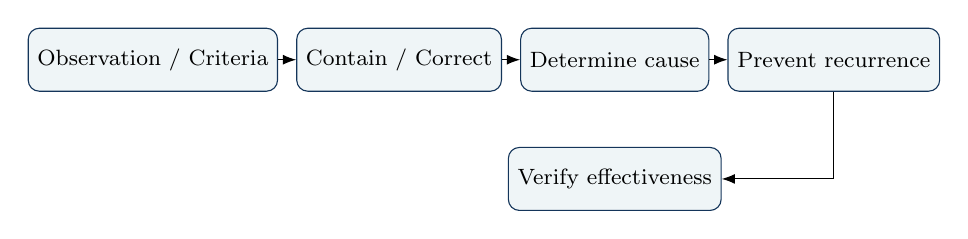
\begin{tikzpicture}[>=Latex, node distance=.23cm, every node/.style={font=\footnotesize}, b/.style={draw=navy,rounded corners,fill=pale,align=center,minimum width=2.15cm,minimum height=.8cm}]
\node[b](a){Observation / Criteria};\node[b,right=of a](b){Contain / Correct};\node[b,right=of b](c){Determine cause};\node[b,right=of c](d){Prevent recurrence};\node[b,below=.7cm of c](e){Verify effectiveness};\draw[->](a)--(b);\draw[->](b)--(c);\draw[->](c)--(d);\draw[->](d.south)|-(e.east);\end{tikzpicture}\end{center}
\section{Management review input pack}
\small\rowcolors{2}{pale}{white}\begin{longtable}{p{.32\linewidth}p{.62\linewidth}}
\rowcolor{navy} \textcolor{white}{\textbf{Input}} & \textcolor{white}{\textbf{Representative evidence}}\\
\endfirsthead
\rowcolor{navy} \textcolor{white}{\textbf{Input}} & \textcolor{white}{\textbf{Representative evidence}}\\
\endhead
Previous actions & Closed/open decisions and overdue items\\
Context and stakeholders & Material change and obligation log\\
Performance and objectives & Validated KPIs and trends\\
Audit/nonconformity & Independent findings and corrective actions\\
Risk assessment and treatment & Risk heat map, accepted residual exposure, SoA status\\
Improvement opportunities & Resource requests and prioritized proposals\\
\end{longtable}\normalsize

\section{Audit readiness quality gates}
\begin{itemize}
\item No ISO wording should be inferred from a tool finding alone; keep the exact source clause available to the assessor.
\item A policy being written is design evidence; verify publication, comprehension and actual operation.
\item A scanned repository does not demonstrate control of unscanned repos, binaries or deployments.
\item Documented information is protected and retained according to the documented process.
\item Report unknown coverage, unsupported systems and stale telemetry explicitly rather than marking compliant.
\end{itemize}

\clearpage\section*{Source and interpretation policy}
\addcontentsline{toc}{section}{Source and interpretation policy}
\textbf{Source editions:} ISO/IEC 27000:2018 (overview and vocabulary); ISO/IEC 27001:2022 (requirements and normative Annex A); ISO/IEC 27002:2022 corrected 2022-03 (control guidance). Specific clause identifiers are references to the supplied editions, not reproduced control text.\par
\textbf{Interpretation:} ``Source-grounded paraphrase'' describes a concept in the cited source. ``Engineering recommendation'' is a practical model, technology choice, owner, evidence example, frequency, template or scoring convention authored for this suite; it is not a claim that ISO prescribes that exact approach.\par
\textbf{Conformity:} Clauses 4--10 of ISO/IEC 27001 govern ISMS conformity. Applicability of controls is determined through risk treatment, with Annex A used as a completeness cross-check and exclusions justified in the Statement of Applicability (SoA). Source documents alone neither certify an ISMS nor prove control operating effectiveness.\par
\textbf{Source licensing:} Do not distribute or embed the licensed standard PDFs in repositories or distribute copied normative text. Review the editions, amendments, and certification scheme applicable to each assessment before relying on this work.\par
\end{document}
